\begin{frame}
\frametitle{Objectives}

To provide tools for representating and analysing any one-dimensional discrete structures.
% in a generic framework. 

\alert{Constant structures, not mutable} 

  \begin{block}{What ?}
    \begin{itemize}
    \item digital curves
      \begin{itemize}
      \item 2d, 3d, nd
      \item 4-connected, 8-connected, disconnected
      \item pixels, interpixels, points
      \item open or closed
      \end{itemize}
		\item chain codes
    \end{itemize}
  \end{block}

  \begin{block}{How ?}
    Segmentation into ``meaningful parts'' (overlapping or not).
  \end{block}


\end{frame}

\begin{frame}
\frametitle{Main applications}

  \begin{block}{What ?}
    \begin{itemize}
    \item<1> polygonal simplification
    \item<1-> estimation 
      \begin{itemize}
      \item<1> length/area
      \item<2> tangents
      \item<3> curvature sign (convexity/concavity)
      \item<4> curvature
      \end{itemize}
    \end{itemize}
  \end{block}

%illustrations
\only<1>{
 \begin{center}
   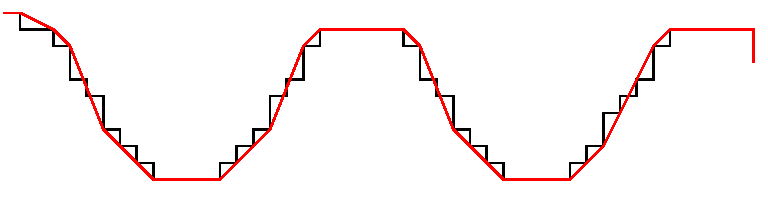
\includegraphics[width=0.8\textwidth]{FP}
 \end{center}
}
\only<2>{
 \begin{center}
   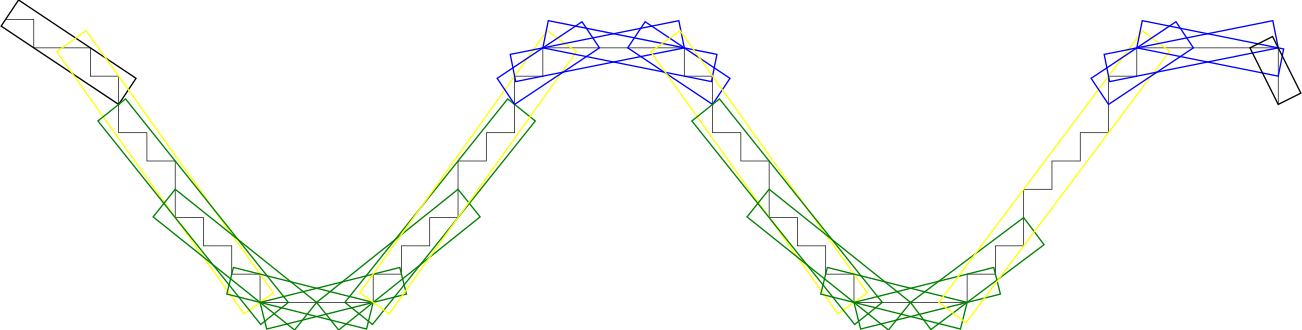
\includegraphics[width=0.8\textwidth]{DSSs}
 \end{center}
}
\only<3>{
 \begin{center}
   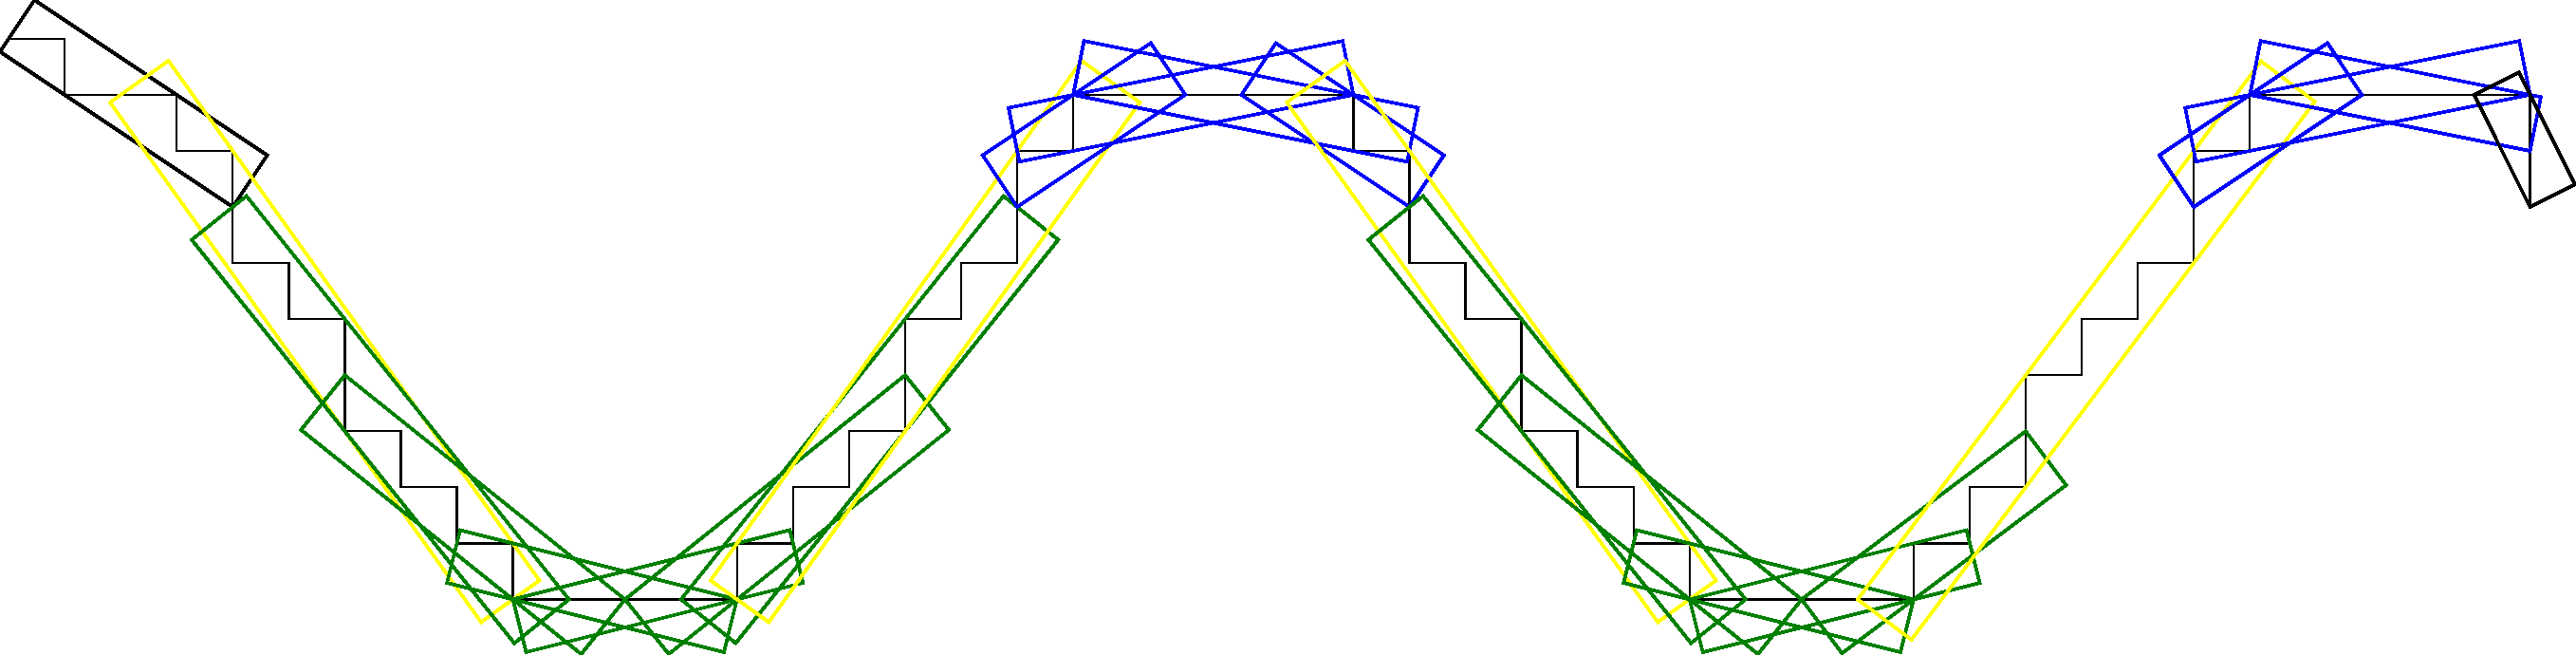
\includegraphics[width=0.8\textwidth]{CCPs}
 \end{center}
}
\only<4>{
 \begin{center}
   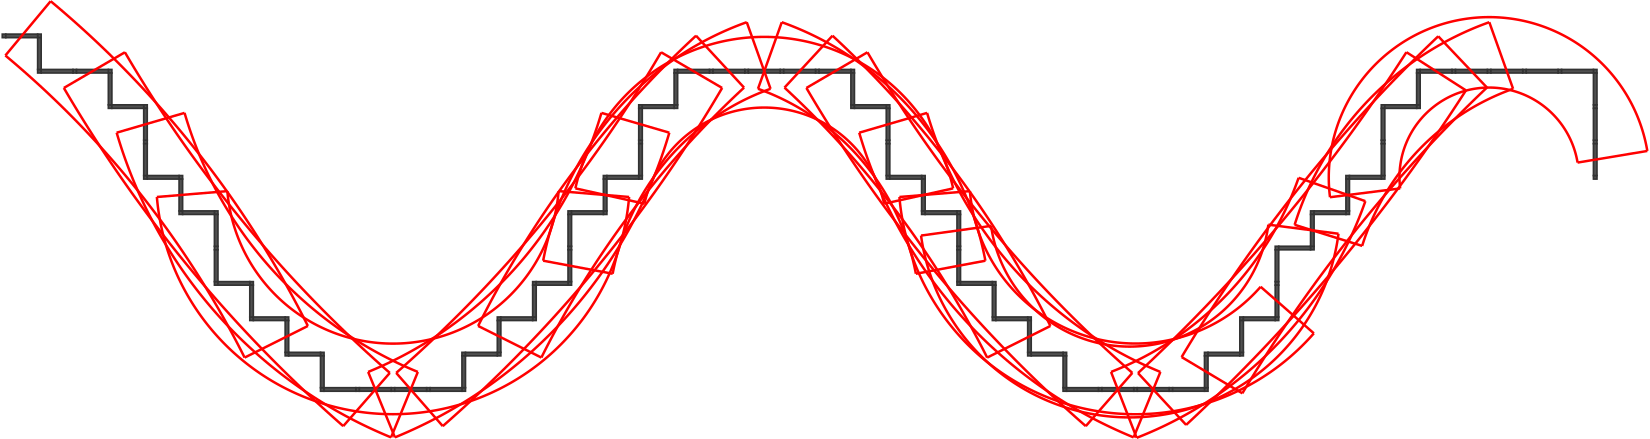
\includegraphics[width=0.8\textwidth]{DCAs}
 \end{center}
}

\end{frame}

\section{Iterators/Circulators and Ranges}


\begin{frame}
  \frametitle{Structures}

  \begin{block}{2 characteristics}
    \begin{itemize}
		\item discrete
    \item one-dimensional
    \end{itemize}
  \end{block}

  \begin{block}{2 notions}
    \begin{itemize}
    \item element
    \item local order (next and previous element)
    \end{itemize}
  \end{block}



\end{frame}

\begin{frame}
  \frametitle{Iterators/Ranges}

  \begin{block}{(Bidirectional) Iterator}
    \begin{itemize}
    \item operator* (to get the element)
    \item operator++, operator- - (to point to the next and previous element)
    \end{itemize}
  \end{block}

  \begin{block}{Reachability}
An iterator j is reachable from an iterator i if and only if i can be made equal to j with finitely many applications of the operator++. 
  \end{block}

  \begin{block}{Range}
If j is reachable from i, one can iterate over the range of elements bounded by i and j, from the one pointed to by i and up to but not including the one pointed to by j. Such a range is valid and is denoted by [i,j).
  \end{block}

\end{frame}

\begin{frame}[containsverbatim]
  \frametitle{Open/Linear structures}

  \begin{block}{Classic(STL) iterators}
\begin{itemize}
  \item past-the-end value
  \item $[begin,end)$ is the whole range
  \item $[i,j)$ is not always valid
  \item $[i,i)$ is the empty range
\end{itemize}
  \end{block}

%\only<1>{
%image
 \begin{center}
   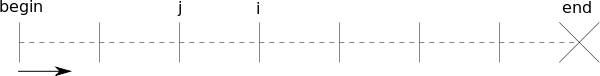
\includegraphics[width=1\textwidth]{linearRange}
 \end{center}
%}

%\only<2>{
  \begin{lstlisting}
typedef DGtal::IteratorCirculatorTraits<Iterator>::Value Value; 
for ( Iterator it = begin; it != end; ++it )
  {
    Value v = *it; 
    ...
  }
  \end{lstlisting}
%}
\end{frame}

\begin{frame}[containsverbatim]
  \frametitle{Adpaters}

TIterator is at least a model of bidirectional iterator

\begin{block}{STL}
 \begin{itemize}
  \item std::reverse\_iterator<TIterator> (for backward scanning)
 \end{itemize}
\end{block}

\begin{block}{in DGtal/base}
 \begin{itemize}
  \item Circulator<TIterator> (CGAL like circular iterator for closed/circular structures)
  \item ConstIteratorAdapter<TIterator, TFunctor, TReturnType>
  \item ConstRangeAdapter<TIterator, TFunctor, TReturnType>
 \end{itemize}
\end{block}

\end{frame}


